\newpage
\section{Theoretical Analysis}
\label{sec:analysis}

In this section we will discuss the theoretical analysis of our circuit, represented in figure \ref{fig:circuit}. For this purpose, we will first explain seperately the Gain stage and the output stage circuits on the Audio Amplifier circuit. The values used throughout this analysis are shown below. 

\begin{table}[h]
    \centering
    \begin{tabular}{|l|c|}
    \hline
    {\bf Symbol} & {\bf Value} \\ \hline
    $R_{S}$ & $100\Omega$ \\ \hline
    $A_f$ & $12 V$ \\ \hline
    $Audio IN Max$ & $10 mV$  \\ \hline
    $Speaker$ & $8 \Omega$\\ \hline
    \end{tabular}
    \caption{Values for theoretical analysis}
    \label{tab:values}
\end{table}


\subsection{Gain Stage}
\label{sec:gain}


The first stage we will discuss is the Gain Stage, which the objetive is to amplify the voltage input signal. Having a high input impedance and a high gain, this stage will have a high output impedance that makes it so there is degradation of the signal in the exit when connecting to a speaker, making it necessary an output stage, that will be explained in the next subsection. Here we used the theoretical model explained in the lectures. The explanation for both this stage and the output stage is already done in the Simulation Analysis section.

In the following table we have the values for the gain, input and output impedances in this stage.


\begin{table}[h]
    \centering
    \begin{tabular}{|l|c|}
    \hline
    {\bf Parameter} & {\bf Value} \\ \hline \hline
    Voltage Gain ($\frac{V_{o}}{V_{i}}$)  & 95.221 \\ \hline
    Input Impedance & 843.98 \\ \hline
    Output Impedance  & 528.99 \\ \hline
    \end{tabular}
    \caption{Values for gain and impedances in Gain Stage.}
    \label{tab:values}
\end{table}


\subsection{Output Stage}
\label{sec:output}


In this output stage, we will have a low output impedance. Because of this, these two stages can now be connected without significant signal loss since the output stage input impedance is higher than the output impedance of the gain stage. The gain of this stage will also be close to one, with prevents signal amplification or attenuation.

Similar to the previous subsection, in the following table we have the values for the gain, input and output impedances in this stage.

\begin{table}[h]
    \centering
    \begin{tabular}{|l|c|}
    \hline
    {\bf Parameter} & {\bf Value} \\ \hline \hline
    Voltage Gain ($\frac{V_{o}}{V_{i}}$)  & 0.98308\\ \hline
    Input Impedance & 16308\\ \hline
    Output Impedance  & 1.1935  \\ \hline
    \end{tabular}
    \caption{Values for gain and impedances in Ouput Stage.}
    \label{tab:values}
\end{table}

To compute the lower cutoff frequency and the gain, we used the following incremental model.

\begin{figure}[ht!] \centering
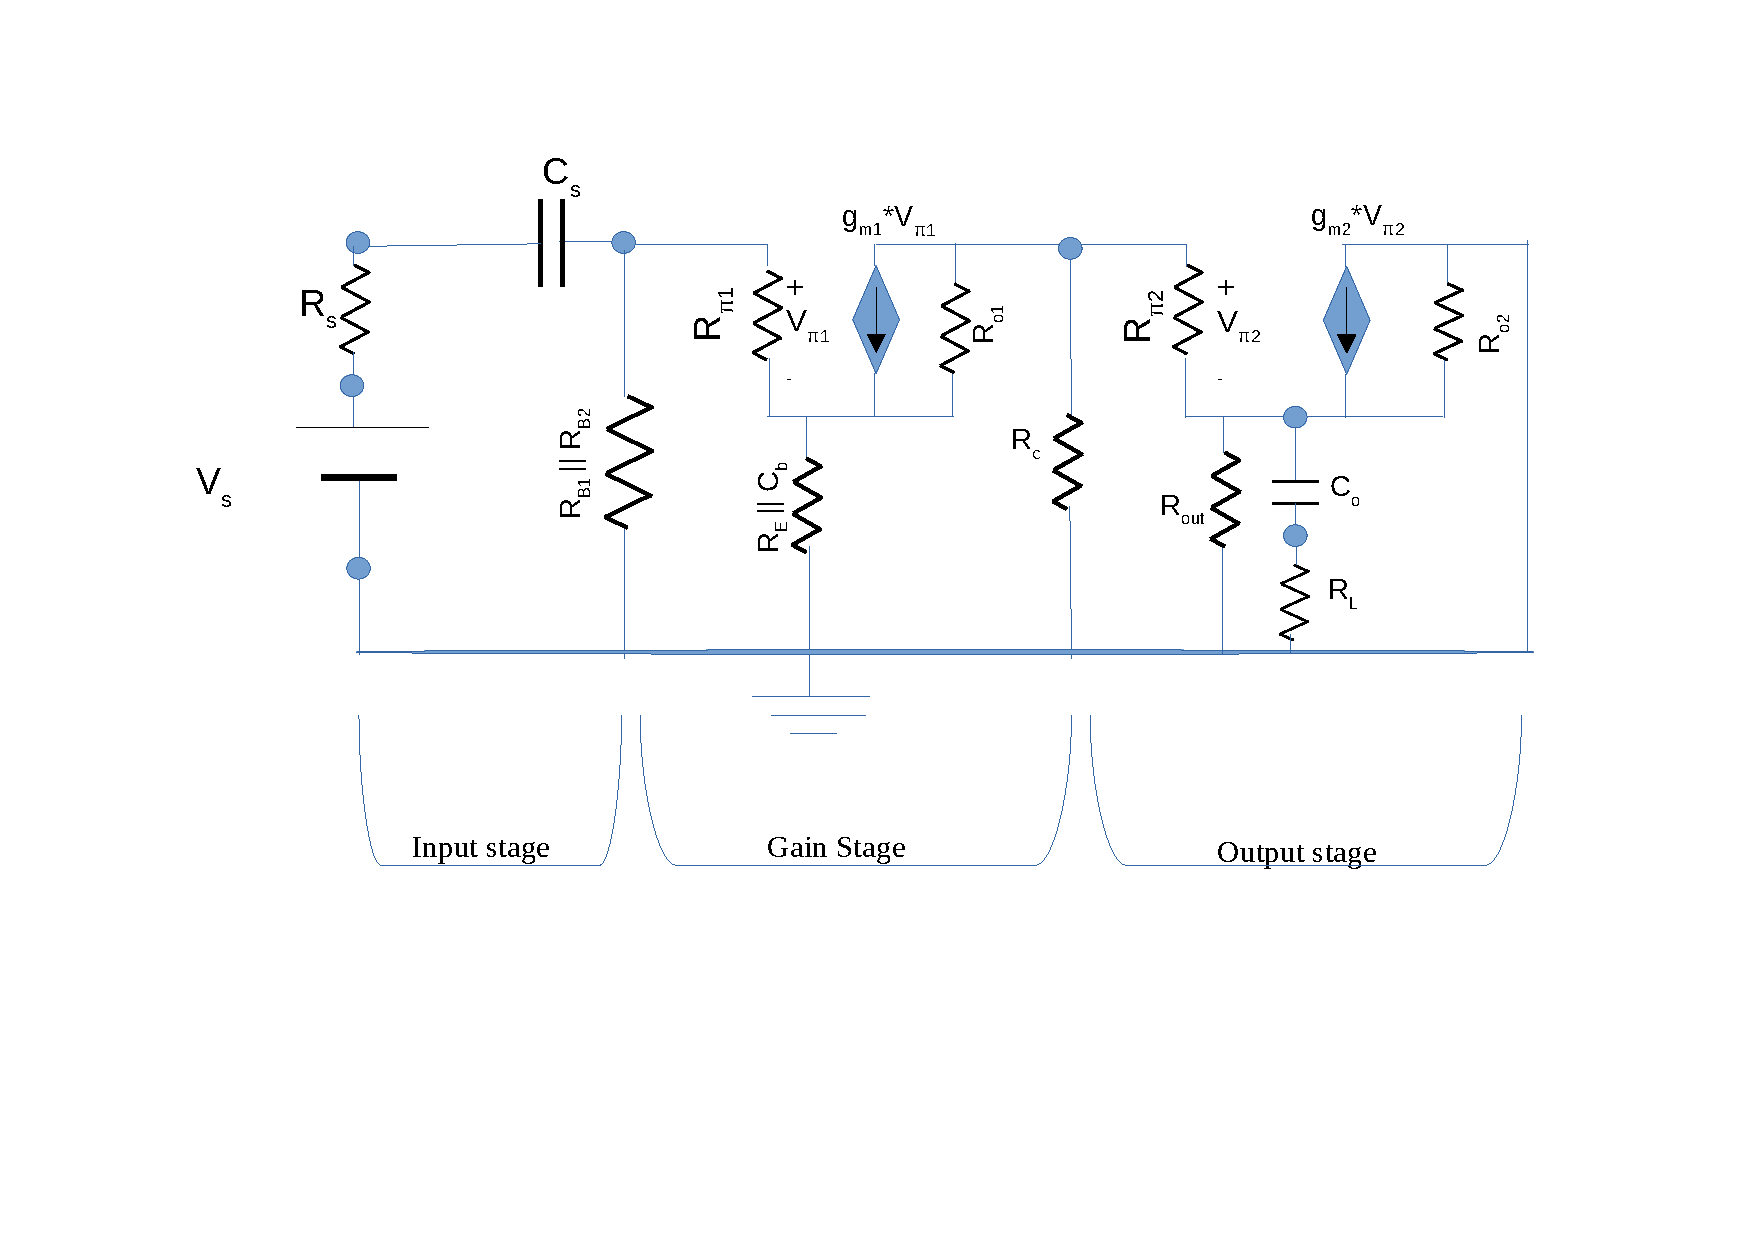
\includegraphics[width=0.95\linewidth]{Incremental_T4.pdf}

\caption{Diagram of the incremental model considered for the gain and frequency response computations.}
\label{fig:diagram_t4}
\end{figure}



In figure we have the plot for the frequency response $V_o$(f)/$V_i$(f) using the incremental circuit, solving the circuit for a frequency vector in log scale with 10 points per decade, from 10Hz to 100MHz.

Below are the total values:

\begin{table}[h]
    \centering
    \begin{tabular}{|l|c|}
    \hline
    {\bf Parameter} & {\bf Value} \\ \hline \hline
    Voltage Gain ($\frac{V_{o}}{V_{i}}$)  & 91.805 \\ \hline
    Input Impedance & 843.98 \\ \hline
    Output Impedance  & 3.3993 \\ \hline
    \end{tabular}
    \caption{Values for gain and impedances in the total circuit}
    \label{tab:values}
\end{table}


  





